\chapter{Kết quả thực nghiệm}
\label{chap:ket-qua}

Mọi con số trong chương là phần trăm (Acc@$k$) hoặc điểm phần trăm ($\Delta$), sinh tự động từ dữ liệu; khoảng trong
ngoặc vuông là khoảng tin cậy \ConstCiLevel\% bootstrap theo cụm khuôn mẫu. Có khoảng hai mươi phép so sánh như vậy và
nhóm không hiệu chỉnh đa so sánh, nên các khoảng sát 0 cần được đọc thận trọng.

\section{RQ1 -- Tái hiện và kiểm tra cách đánh giá}
\label{sec:rq1}

\subsection{Tái hiện và hai cách chấm điểm}

Tính lại từ nhật ký công bố khớp từng con số của cả 13 cấu hình trong bảng kết quả của SemLoc. \emph{Chạy lại} SemLoc với
chính mô hình của bài báo (Claude Sonnet 4.6) trên tập dev thì không khớp: Acc@1 \RepClaudeDevRerunAccOne\% và Acc@3
\RepClaudeDevRerunAccThree\% so với \RepClaudeDevPublishedAccOne\% và \RepClaudeDevPublishedAccThree\% trong nhật ký trên
cùng các chương trình; ràng buộc sinh ra ít bị vi phạm trong kiểm thử thất bại hơn, và nhóm không tìm thấy nguyên nhân
ở hạ tầng của mình.

Bảng~\ref{tab:rq1} so sánh cách chấm của tác giả với cách chấm công bằng. Ba điểm nổi bật:
\begin{itemize}
\item \textbf{Gỡ lỗi chia đôi}: mã chấm điểm công bố cho \RqOneDdAuthorAllAccOne\% (mọi lần trúng tính là hạng 1), trong
khi bài báo ghi 0 và cách chấm công bằng cho \RqOneDdFairAllAccOne\%, vì phương pháp này không xếp hạng dòng nào.
\item \textbf{SBFL bị đánh giá thấp ở top-5}: Acc@5 của Ochiai là \RqOneSbflOchiaiAuthorAllAccFive\% theo cách của tác giả
và \RqOneSbflOchiaiFairAllAccFive\% khi dùng hạng trung bình.
\item \textbf{SemLoc} gần như không đổi khi chấm công bằng, nhưng \textbf{bỏ điểm thưởng cho dòng LLM tự đoán} --- thành
phần không có trong bài báo --- làm Acc@1 giảm từ \RqOneSemlocClaudeTZeroEightFairAllAccOne\% xuống
\RqOneSemlocClaudeTZeroEightNoPriorFairAllAccOne\% (Claude) và từ \RqOneSemlocGeminiTZeroEightFairAllAccOne\% xuống
\RqOneSemlocGeminiTZeroEightNoPriorFairAllAccOne\% (Gemini).
\end{itemize}

\begin{table}[H]
\centering
\caption{Kết quả công bố tính lại theo hai cách chấm (nhật ký của tác giả, 250 chương trình)}
\label{tab:rq1}
\resizebox{\linewidth}{!}{\begin{tabular}{lrrrrrr}
\toprule
 & \multicolumn{3}{c}{Cách chấm của tác giả} & \multicolumn{3}{c}{Cách chấm công bằng} \\
\cmidrule(lr){2-4}\cmidrule(lr){5-7}
Cấu hình (cả 250 chương trình) & Acc@1 & Acc@3 & Acc@5 & Acc@1 & Acc@3 & Acc@5 \\
\midrule
SemLoc, Claude Sonnet 4,6, $T{=}0,8$ & 42,8 & 68,0 & 76,8 & 42,8 & 65,6 & 76,8 \\
SemLoc, Gemini 2,5 Pro, $T{=}0,8$ & 39,8 & 64,7 & 73,5 & 39,6 & 64,4 & 72,8 \\
SemLoc Claude $T{=}0,8$ không có điểm thưởng dòng đoán & -- & -- & -- & 30,0 & 55,6 & 66,4 \\
SemLoc Gemini $T{=}0,8$ không có điểm thưởng dòng đoán & -- & -- & -- & 27,2 & 55,6 & 64,0 \\
SemLoc không CF (lượt chạy riêng), Claude & 30,8 & 59,6 & 68,8 & -- & -- & -- \\
LLM hỏi thẳng, Claude & 35,2 & 41,2 & 41,2 & 35,2 & 41,2 & 41,2 \\
SBFL Ochiai & 6,4 & 13,2 & 30,4 & 4,0 & 16,0 & 48,0 \\
SBFL DStar (tính lại) & -- & -- & -- & 4,0 & 16,0 & 48,0 \\
Gỡ lỗi chia đôi (DD) & 38,0 & 38,0 & 38,0 & 0,0 & 0,0 & 0,0 \\
\bottomrule
\end{tabular}
}
\end{table}

\subsection{Kiểm chứng phản thực tế và lỗi của gói mã công bố}

Trong mã nguồn công bố, kết quả của bước kiểm chứng phản thực tế được tính ra nhưng \emph{không dùng để xếp hạng}:
thứ hạng có và không có bước này trùng nhau ở cả 250 chương trình của cả năm cấu hình có dữ liệu. Con số ``không có kiểm
chứng phản thực tế'' trong bài báo đến từ một lượt chạy riêng không công bố điểm từng chương trình; Acc@1 của nó
(\RqOneCfDisabledClaudeTZeroEightAuthorAllAccOne\%) gần bằng SemLoc khi bỏ điểm thưởng, gợi ý một khác biệt về cấu hình
hơn là tác dụng của bước này, nhưng nhóm không xác định được. Bộ chạy BugsInPy của SemLoc có thêm hai lỗi: (i) chỉ số
``hạng tốt nhất'' nó báo cáo là hạng của \emph{chính dòng LLM đoán}, không phải của dòng lập trình viên đã sửa; (ii) bước
vá thử sửa tệp nguồn rồi khôi phục trong cùng một giây với cùng kích thước tệp, để lại bản biên dịch Python
(\texttt{.pyc}) của phiên bản \emph{đã vá}, khiến lỗi ``biến mất'' ở lượt chạy sau. Nhóm đã sửa lỗi thứ hai trong bộ chạy
của mình và chấm lại BugsInPy theo dòng đã sửa thật.

\subsection{Ảnh hưởng của dòng lỗi chuẩn}

Trên lượt chạy của nhóm, chuyển từ dòng lỗi chuẩn gốc (200 chương trình) sang bộ đã sửa (179 chương trình) làm Acc@1 của
SemLoc tăng từ \RqTwoOriginalAllSemlocAccOneMean\% lên \RqTwoRepairedAllSemlocAccOneMean\%. Một phần của mức tăng này là do
mẫu số nhỏ hơn: bộ đã sửa bỏ các lỗi không kiểm chứng được. Chỉ tính các lỗi được kiểm thử thất bại chạy tới trên bộ
gốc, SemLoc đã đạt \RqTwoOriginalExecutableSemlocAccOneMean\%. SBFL tăng ít hơn nhiều (Acc@3 từ
\RqTwoOriginalAllSbflOchiaiAccThreeMean\% lên \RqTwoRepairedAllSbflOchiaiAccThreeMean\%).

\section{RQ2 -- Cải tiến và đối chứng}
\label{sec:rq2}

\subsection{Một prompt và quy trình nhiều bước}

Bảng~\ref{tab:rq2} là kết quả trên 200 chương trình của tập test, ba lần chạy Gemini 3.8 Flash. Kết quả phụ thuộc vào việc
lỗi có được kiểm thử thất bại chạy tới hay không. \textbf{Trên các lỗi được chạy tới}, LLM + độ phủ hơn SemLoc ở Acc@3
\RqTwoOriginalExecutableLlmCoverageDAccThree{} điểm [\RqTwoOriginalExecutableLlmCoverageDAccThreeLo;
\RqTwoOriginalExecutableLlmCoverageDAccThreeHi] trên bộ dòng lỗi chuẩn gốc (148 chương trình) và
\RqTwoRepairedAllLlmCoverageDAccThree{} điểm [\RqTwoRepairedAllLlmCoverageDAccThreeLo;
\RqTwoRepairedAllLlmCoverageDAccThreeHi] trên bộ đã sửa. \textbf{Trên toàn bộ nhãn gốc}, gồm cả lỗi không kiểm thử nào
chạy tới, mức hơn chỉ còn \RqTwoOriginalAllLlmCoverageDAccThree{} điểm [\RqTwoOriginalAllLlmCoverageDAccThreeLo;
\RqTwoOriginalAllLlmCoverageDAccThreeHi] và SemLoc tốt hơn ở Acc@5 (\RqTwoOriginalAllSemlocAccFiveMean\% so với
\RqTwoOriginalAllLlmCoverageAccFiveMean\%): một prompt dựa trên độ phủ không thể chỉ vào dòng mà không kiểm thử nào chạy
qua. Ở Acc@1, mức hơn (\RqTwoRepairedAllLlmCoverageDAccOne{} [\RqTwoRepairedAllLlmCoverageDAccOneLo;
\RqTwoRepairedAllLlmCoverageDAccOneHi]) chỉ thấy rõ khi gộp ba lần chạy; từng lần riêng chưa đạt ý nghĩa thống kê.
\textbf{LLM hỏi thẳng} (chỉ có mã nguồn) không kém SemLoc ở Acc@1 ($\Delta$ = \RqTwoRepairedAllLlmDirectDAccOne{},
khoảng tin cậy chứa 0) nhưng Acc@3 thay đổi \RqTwoRepairedAllLlmDirectDAccThree{} điểm. Vì LLM + độ phủ thêm cùng lúc kết
quả kiểm thử, thông báo lỗi và độ phủ, khoảng cách này đo tác dụng của bằng chứng thực thi trong prompt nói chung, chưa
tách riêng độ phủ.

\begin{table}[H]
\centering
\caption{RQ2: so sánh trên tập test (Gemini 3.8 Flash, 3 lần chạy; $\Delta$ so với SemLoc)}
\label{tab:rq2}
\resizebox{\linewidth}{!}{\begin{tabular}{lrrrrrr}
\toprule
Phương pháp & Acc@1 & Acc@3 & Acc@5 & $\Delta$Acc@1 [CI 95\%] & $\Delta$Acc@3 [CI 95\%] & $r_{\text{rb}}$ \\
\midrule
\multicolumn{7}{l}{\emph{Ground truth gốc, $n=200$, 3 lần lặp}} \\
SemLoc (bản phát hành) & 36,8{\scriptsize$\pm$0,8} & 60,3{\scriptsize$\pm$2,3} & 75,0{\scriptsize$\pm$0,9} & -- & -- & -- \\
\quad bỏ điểm thưởng dòng đoán & 29,2{\scriptsize$\pm$1,4} & 57,7{\scriptsize$\pm$2,5} & 72,7{\scriptsize$\pm$1,3} & -7,7{\scriptsize\,[-13,9; -1,6]} & -2,7{\scriptsize\,[-4,9; -0,9]} & -0,38 \\
\quad chỉ thưởng khi có căn cứ & 34,7{\scriptsize$\pm$1,5} & 58,2{\scriptsize$\pm$2,9} & 72,8{\scriptsize$\pm$1,5} & -2,2{\scriptsize\,[-4,2; -0,6]} & -2,2{\scriptsize\,[-4,2; -0,6]} & -0,94 \\
\quad + chỉ cổng độ phủ & 36,8{\scriptsize$\pm$0,8} & 57,7{\scriptsize$\pm$1,8} & 62,5{\scriptsize$\pm$1,3} & +0,0{\scriptsize\,[0,0; 0,0]} & -2,7{\scriptsize\,[-7,7; 1,7]} & -0,59 \\
\quad + chỉ $\lambda$·Ochiai & 36,8{\scriptsize$\pm$0,8} & 61,3{\scriptsize$\pm$1,9} & 75,0{\scriptsize$\pm$0,9} & +0,0{\scriptsize\,[0,0; 0,0]} & +1,0{\scriptsize\,[0,2; 2,3]} & +0,54 \\
\quad + xếp lại bằng CF & 35,0{\scriptsize$\pm$1,0} & 62,2{\scriptsize$\pm$2,5} & 77,7{\scriptsize$\pm$1,8} & -1,8{\scriptsize\,[-3,8; -0,3]} & +1,8{\scriptsize\,[0,5; 3,5]} & +0,36 \\
CovGate (nhóm đề xuất) & 36,8{\scriptsize$\pm$0,8} & 61,3{\scriptsize$\pm$1,9} & 75,0{\scriptsize$\pm$0,9} & +0,0{\scriptsize\,[0,0; 0,0]} & +1,0{\scriptsize\,[0,2; 2,3]} & +0,54 \\
CovGate + xếp lại bằng CF & 35,0{\scriptsize$\pm$1,0} & 62,5{\scriptsize$\pm$2,2} & 77,7{\scriptsize$\pm$1,8} & -1,8{\scriptsize\,[-3,8; -0,3]} & +2,2{\scriptsize\,[0,9; 3,8]} & +0,46 \\
LLM hỏi thẳng (1 prompt) & 40,0{\scriptsize$\pm$0,0} & 43,0{\scriptsize$\pm$0,5} & 43,2{\scriptsize$\pm$0,8} & +3,2{\scriptsize\,[-0,8; 7,4]} & -17,3{\scriptsize\,[-23,3; -11,1]} & -0,51 \\
LLM + độ phủ (1 prompt, nhóm đề xuất) & 40,2{\scriptsize$\pm$0,6} & 68,2{\scriptsize$\pm$0,3} & 70,0{\scriptsize$\pm$0,9} & +3,3{\scriptsize\,[0,5; 6,5]} & +7,8{\scriptsize\,[0,2; 15,2]} & +0,04 \\
SBFL Ochiai & 3,0{\scriptsize$\pm$0,0} & 15,5{\scriptsize$\pm$0,0} & 48,0{\scriptsize$\pm$0,0} & -33,8{\scriptsize\,[-41,2; -26,8]} & -44,8{\scriptsize\,[-52,8; -36,6]} & -0,87 \\
\midrule
\multicolumn{7}{l}{\emph{Ground truth đã sửa bằng thực thi, $n=179$, 3 lần lặp}} \\
SemLoc (bản phát hành) & 52,3{\scriptsize$\pm$0,9} & 75,4{\scriptsize$\pm$2,0} & 82,7{\scriptsize$\pm$1,1} & -- & -- & -- \\
\quad bỏ điểm thưởng dòng đoán & 43,2{\scriptsize$\pm$2,1} & 70,8{\scriptsize$\pm$2,3} & 78,4{\scriptsize$\pm$1,7} & -9,1{\scriptsize\,[-16,7; -1,9]} & -4,7{\scriptsize\,[-7,9; -2,1]} & -0,37 \\
\quad chỉ thưởng khi có căn cứ & 48,2{\scriptsize$\pm$1,7} & 71,3{\scriptsize$\pm$2,8} & 78,6{\scriptsize$\pm$2,0} & -4,1{\scriptsize\,[-7,2; -1,7]} & -4,1{\scriptsize\,[-7,2; -1,7]} & -1,00 \\
\quad + chỉ cổng độ phủ & 52,3{\scriptsize$\pm$0,9} & 79,1{\scriptsize$\pm$2,0} & 85,1{\scriptsize$\pm$1,3} & +0,0{\scriptsize\,[0,0; 0,0]} & +3,7{\scriptsize\,[1,5; 6,6]} & +1,00 \\
\quad + chỉ $\lambda$·Ochiai & 52,3{\scriptsize$\pm$0,9} & 79,3{\scriptsize$\pm$1,7} & 85,1{\scriptsize$\pm$1,3} & +0,0{\scriptsize\,[0,0; 0,0]} & +3,9{\scriptsize\,[1,6; 6,8]} & +0,85 \\
\quad + xếp lại bằng CF & 49,9{\scriptsize$\pm$0,9} & 76,2{\scriptsize$\pm$1,8} & 83,4{\scriptsize$\pm$1,4} & -2,4{\scriptsize\,[-4,8; -0,6]} & +0,7{\scriptsize\,[0,0; 2,1]} & -0,35 \\
CovGate (nhóm đề xuất) & 52,3{\scriptsize$\pm$0,9} & 79,3{\scriptsize$\pm$1,7} & 85,1{\scriptsize$\pm$1,3} & +0,0{\scriptsize\,[0,0; 0,0]} & +3,9{\scriptsize\,[1,6; 6,8]} & +0,85 \\
CovGate + xếp lại bằng CF & 49,9{\scriptsize$\pm$0,9} & 77,1{\scriptsize$\pm$2,2} & 85,3{\scriptsize$\pm$1,2} & -2,4{\scriptsize\,[-4,8; -0,6]} & +1,7{\scriptsize\,[0,5; 3,3]} & +0,28 \\
LLM hỏi thẳng (1 prompt) & 56,8{\scriptsize$\pm$0,7} & 62,8{\scriptsize$\pm$0,7} & 62,9{\scriptsize$\pm$0,9} & +4,5{\scriptsize\,[-0,4; 9,7]} & -12,7{\scriptsize\,[-19,7; -6,2]} & -0,28 \\
LLM + độ phủ (1 prompt, nhóm đề xuất) & 57,2{\scriptsize$\pm$0,9} & 92,0{\scriptsize$\pm$0,3} & 93,7{\scriptsize$\pm$0,9} & +4,8{\scriptsize\,[1,5; 8,7]} & +16,6{\scriptsize\,[10,5; 22,8]} & +0,65 \\
SBFL Ochiai & 3,9{\scriptsize$\pm$0,0} & 19,0{\scriptsize$\pm$0,0} & 67,6{\scriptsize$\pm$0,0} & -48,4{\scriptsize\,[-58,6; -38,3]} & -56,4{\scriptsize\,[-67,0; -45,4]} & -0,85 \\
\bottomrule
\end{tabular}
}
\end{table}

\subsection{Theo loại lỗi và từng thành phần của CovGate}

Bảng~\ref{tab:rq2-nhan} tách kết quả theo nhãn lỗi của bộ đã sửa. Phần hơn của LLM + độ phủ không chỉ đến từ các lỗi mà độ
phủ tự làm lộ: trên lỗi ngữ nghĩa thuần --- nơi kiểm thử đạt và không đạt chạy qua cùng dòng --- Acc@3 vẫn là
\RqTwoRepairedSemanticLlmCoverageAccThreeMean\% so với \RqTwoRepairedSemanticSemlocAccThreeMean\%.

\begin{table}[H]
\centering
\caption{RQ2 theo nhãn lỗi (dòng lỗi chuẩn đã sửa)}
\label{tab:rq2-nhan}
\resizebox{\linewidth}{!}{\begin{tabular}{lrrrrrrrrr}
\toprule
 & & \multicolumn{2}{c}{SBFL} & \multicolumn{2}{c}{SemLoc} & \multicolumn{2}{c}{CovGate} & \multicolumn{2}{c}{LLM + độ phủ} \\
\cmidrule(lr){3-4}\cmidrule(lr){5-6}\cmidrule(lr){7-8}\cmidrule(lr){9-10}
Nhãn lỗi & $n$ & Acc@1 & Acc@3 & Acc@1 & Acc@3 & Acc@1 & Acc@3 & Acc@1 & Acc@3 \\
\midrule
Ngữ nghĩa & 162 & 1,8 & 17,3 & 54,7 & 77,6 & 54,7 & 81,1 & 60,1 & 91,8 \\
Lộ qua độ phủ & 17 & 23,5 & 35,3 & 29,4 & 54,9 & 29,4 & 62,7 & 29,4 & 94,1 \\
Thực thi được (trừ nhóm không thực thi) & 179 & 3,9 & 19,0 & 52,3 & 75,4 & 52,3 & 79,3 & 57,2 & 92,0 \\
\bottomrule
\end{tabular}
}
\end{table}

CovGate được chọn trên tập dev là một bước phá hòa bằng Ochiai (mục~\ref{sec:phuong-phap-so-sanh}); nó thay đổi Acc@3
\RqTwoRepairedAllCovgateDAccThree{} điểm [\RqTwoRepairedAllCovgateDAccThreeLo; \RqTwoRepairedAllCovgateDAccThreeHi] trên bộ
đã sửa và \RqTwoOriginalAllCovgateDAccThree{} điểm [\RqTwoOriginalAllCovgateDAccThreeLo;
\RqTwoOriginalAllCovgateDAccThreeHi] trên bộ gốc, không đổi Acc@1. Riêng cổng độ phủ cho mức tăng tương tự trên bộ đã
sửa nhưng thay đổi Acc@3 \RqTwoOriginalAllGateOnlyDAccThree{} điểm trên bộ gốc, vì nó loại mọi lỗi không được chạy tới.
``Chỉ thưởng khi có căn cứ'' thay đổi Acc@1 \RqTwoRepairedAllGroundedPriorOnlyDAccOne{} điểm và xếp lại bằng kiểm chứng
phản thực tế thay đổi \RqTwoRepairedAllCfRerankDAccOne{} điểm: bằng chứng thực thi không phân biệt được dòng đoán đúng với
dòng đoán sai.

\subsection{Grounded hay guessed: giá trị biên và phân rã}

Vì điểm thưởng lớn hơn mọi điểm ràng buộc, thêm phổ vào dòng đoán \emph{không thể} thay đổi dòng đầu tiên: riêng dòng đoán
và SemLoc cùng đạt Acc@1 \RqTwoRepairedAllSemlocAccOneMean\%, còn riêng phổ đạt \RqTwoRepairedAllSemlocNoPriorAccOneMean\%.
Giá trị Shapley của phổ ở Acc@1 (Bảng~\ref{tab:phan-ra}, \DecSemlocRepairedAllAccOnePhiSpectrum{} điểm) vì vậy là phần
công cho điều phổ \emph{sẽ} đạt được nếu không có dòng đoán, không phải đóng góp vào dòng đầu của SemLoc. Ở top-3, phổ có
tác dụng thật: dòng đoán chỉ nêu một dòng nên dừng ở \RqTwoRepairedAllSemlocAccOneMean\%, riêng phổ đạt
\RqTwoRepairedAllSemlocNoPriorAccThreeMean\%, và cả hai cùng đạt \RqTwoRepairedAllSemlocAccThreeMean\%. Kết luận:
\textbf{hạng 1 là ``guessed'' theo thiết kế, top-3 là nơi bằng chứng thực thi có tác dụng}. Trên nhật ký của tác giả
(Claude), phân rã cho \PubSemlocClaudeTZeroEightSemlocOriginalAllAccOneFull\% =
\PubSemlocClaudeTZeroEightSemlocOriginalAllAccOnePhiGuess{} (dòng đoán) +
\PubSemlocClaudeTZeroEightSemlocOriginalAllAccOnePhiSpectrum{} (phổ).

\begin{table}[H]
\centering
\caption{Phân rã Shapley độ chính xác của SemLoc (lượt chạy của nhóm, 3 lần)}
\label{tab:phan-ra}
\resizebox{\linewidth}{!}{\begin{tabular}{llrrrrr}
\toprule
Dòng lỗi chuẩn & Chỉ số & Tổng & Dòng LLM đoán & Phổ ngữ nghĩa & Độ phủ & CF \\
\midrule
\multicolumn{7}{l}{\emph{SemLoc như phát hành (dòng đoán + phổ)}} \\
Bản gốc ($n=200$) & Acc@1 & 36,8 & 22,2{\scriptsize\,[16,5; 28,4]} & 14,6{\scriptsize\,[11,8; 17,5]} & -- & -- \\
Bản gốc ($n=200$) & Acc@3 & 60,3 & 19,8{\scriptsize\,[16,1; 23,8]} & 40,6{\scriptsize\,[35,6; 45,3]} & -- & -- \\
Đã sửa ($n=179$) & Acc@1 & 52,3 & 30,7{\scriptsize\,[23,5; 37,8]} & 21,6{\scriptsize\,[17,4; 26,1]} & -- & -- \\
Đã sửa ($n=179$) & Acc@3 & 75,4 & 28,5{\scriptsize\,[23,4; 33,5]} & 46,9{\scriptsize\,[41,9; 51,7]} & -- & -- \\
\midrule
\multicolumn{7}{l}{\emph{Mọi tín hiệu (+ Ochiai thô, + xếp lại bằng CF)}} \\
Bản gốc ($n=200$) & Acc@1 & 35,0 & 22,7{\scriptsize\,[17,4; 28,3]} & 12,5{\scriptsize\,[10,0; 15,2]} & -0,5{\scriptsize\,[-1,5; 0,6]} & 0,3{\scriptsize\,[-0,6; 1,1]} \\
Bản gốc ($n=200$) & Acc@3 & 59,0 & 17,6{\scriptsize\,[14,2; 21,4]} & 35,8{\scriptsize\,[31,6; 40,2]} & 4,6{\scriptsize\,[0,1; 9,0]} & 1,1{\scriptsize\,[0,5; 1,8]} \\
Đã sửa ($n=179$) & Acc@1 & 49,9 & 31,9{\scriptsize\,[25,3; 38,5]} & 18,6{\scriptsize\,[14,4; 22,9]} & -1,1{\scriptsize\,[-2,3; 0,2]} & 0,5{\scriptsize\,[-0,7; 1,5]} \\
Đã sửa ($n=179$) & Acc@3 & 80,6 & 25,9{\scriptsize\,[20,8; 31,0]} & 44,4{\scriptsize\,[39,7; 49,3]} & 9,4{\scriptsize\,[5,8; 13,4]} & 0,9{\scriptsize\,[0,3; 1,7]} \\
\bottomrule
\end{tabular}
}
\end{table}

\subsection{Chi phí}

SemLoc tốn trung bình \CostSemlocTokensK{} nghìn token cho mỗi chương trình, trong đó bước kiểm chứng phản thực tế chiếm
\CostCfSharePct\% số lượt gọi LLM mà không cải thiện thứ hạng; LLM + độ phủ chỉ tốn \CostLlmCoverageTokensK{} nghìn
token. Hình~\ref{fig:pareto} đặt độ chính xác cạnh chi phí cho năm mô hình trên cùng một tập con
(\ParetoSemlocGeminiThreeEightFlashN{} chương trình): với mọi mô hình, LLM + độ phủ có Acc@3 cao hơn và tốn ít token hơn
SemLoc. Các so sánh theo từng mô hình chưa có khoảng tin cậy; ở Acc@1, GPT-6 luna không hơn, và trên tập con này LLM hỏi
thẳng có Acc@1 cao nhất với Gemini 3.8 Flash (\ParetoLlmDirectGeminiThreeEightFlashAccOne\% so với
\ParetoLlmCoverageGeminiThreeEightFlashAccOne\%).

\begin{figure}[H]
\centering
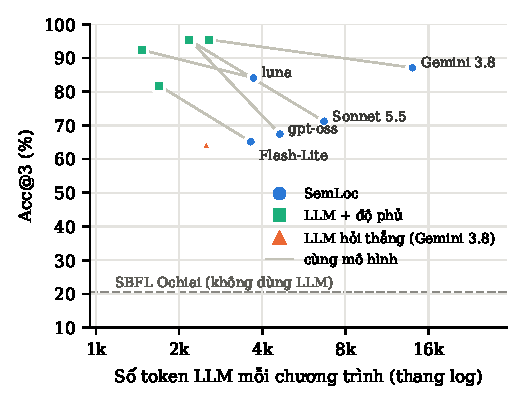
\includegraphics[width=0.75\linewidth]{../generated/vi/pareto.pdf}
\caption{Chi phí và độ chính xác (Acc@3) trên cùng tập con, dòng lỗi chuẩn đã sửa; đường nối hai phương pháp của cùng một
mô hình}
\label{fig:pareto}
\end{figure}

\section{RQ3 -- Độ bền}
\label{sec:rq3}

\subsection{Lỗi thật BugsInPy}

Bảng~\ref{tab:rq3-bip} cho kết quả trên 31 lỗi của một dự án (youtube-dl), ba lần chạy. Theo thiết kế, dòng đầu của SemLoc
là dòng LLM đoán, nên Acc@1 của SemLoc chính là của dòng đoán (\BipAllLlmGuessAccOneMean\%); riêng phổ ngữ nghĩa chỉ đặt
đúng \BipAllSemlocSpectrumAccOneMean\% ở hạng 1, gần SBFL (\BipAllSbflOchiaiAccOneMean\%). LLM + độ phủ đi cùng chiều với
kết quả trên SemFault-250 --- Acc@3 \BipAllLlmCoverageAccThreeMean\% so với \BipAllSemlocPriorAccThreeMean\% --- nhưng với
31 lỗi, khoảng tin cậy [\BipAllLlmCoverageDAccThreeLo; \BipAllLlmCoverageDAccThreeHi] vẫn chứa 0. ``Lỗi được chạy tới'' là
các lỗi có kiểm thử thất bại chạy qua một dòng lỗi chuẩn; chỉ số của gói mã công bố (dòng cuối bảng) là hạng của dòng LLM
đoán, đo mức nhất quán của LLM với chính nó chứ không đo khả năng định vị.

\begin{table}[H]
\centering
\caption{RQ3a: 31 lỗi thật youtube-dl (BugsInPy), 3 lần chạy}
\label{tab:rq3-bip}
\resizebox{\linewidth}{!}{\begin{tabular}{lrrrrr}
\toprule
 & \multicolumn{3}{c}{Mọi lỗi ($n=31$)} & \multicolumn{2}{c}{Lỗi được chạy tới ($n=26$)} \\
\cmidrule(lr){2-4}\cmidrule(lr){5-6}
Phương pháp & Acc@1 & Acc@3 & Acc@5 & Acc@1 & Acc@3 \\
\midrule
Chỉ phổ ngữ nghĩa của SemLoc & 7,5{\scriptsize$\pm$1,9} & 29,0{\scriptsize$\pm$3,2} & 37,6{\scriptsize$\pm$3,7} & 9,0{\scriptsize$\pm$2,2} & 34,6{\scriptsize$\pm$3,9} \\
SemLoc (phổ + điểm thưởng dòng đoán) & 46,2{\scriptsize$\pm$6,7} & 53,8{\scriptsize$\pm$7,4} & 55,9{\scriptsize$\pm$6,7} & 51,3{\scriptsize$\pm$8,0} & 60,3{\scriptsize$\pm$8,9} \\
Chỉ dòng LLM đoán & 46,2{\scriptsize$\pm$6,7} & 46,2{\scriptsize$\pm$6,7} & 46,2{\scriptsize$\pm$6,7} & 51,3{\scriptsize$\pm$8,0} & 51,3{\scriptsize$\pm$8,0} \\
CovGate (nhóm đề xuất) & 46,2{\scriptsize$\pm$6,7} & 54,8{\scriptsize$\pm$6,5} & 57,0{\scriptsize$\pm$7,4} & 51,3{\scriptsize$\pm$8,0} & 61,5{\scriptsize$\pm$7,7} \\
LLM + độ phủ (1 prompt, nhóm đề xuất) & 51,6{\scriptsize$\pm$5,6} & 69,9{\scriptsize$\pm$3,7} & 75,3{\scriptsize$\pm$1,9} & 59,0{\scriptsize$\pm$5,9} & 75,6{\scriptsize$\pm$4,4} \\
SBFL Ochiai & 9,7{\scriptsize$\pm$0,0} & 29,0{\scriptsize$\pm$0,0} & 29,0{\scriptsize$\pm$0,0} & 11,5{\scriptsize$\pm$0,0} & 34,6{\scriptsize$\pm$0,0} \\
SBFL DStar & 9,7{\scriptsize$\pm$0,0} & 29,0{\scriptsize$\pm$0,0} & 29,0{\scriptsize$\pm$0,0} & 11,5{\scriptsize$\pm$0,0} & 34,6{\scriptsize$\pm$0,0} \\
\midrule
Chỉ số của gói mã công bố (hạng của dòng LLM đoán) & 39,8{\scriptsize$\pm$1,9} & 45,2{\scriptsize$\pm$3,2} & 51,6{\scriptsize$\pm$3,2} & 37,2{\scriptsize$\pm$2,2} & 43,6{\scriptsize$\pm$5,9} \\
\bottomrule
\end{tabular}
}
\end{table}

\subsection{Đổi tên định danh}

Bảng~\ref{tab:rq3-ren} so sánh từng chương trình với bản đổi tên của nó, theo cặp lần chạy (chỉ với Gemini 3.8 Flash). Dòng
LLM đoán không thay đổi đáng kể (Acc@1 $\Delta$ = \RenRepairedLlmGuessDAccOne{} [\RenRepairedLlmGuessDAccOneLo;
\RenRepairedLlmGuessDAccOneHi]), nên không có dấu hiệu mô hình đoán nhờ nhớ tên. Ngược lại, phổ vi phạm ràng buộc cần tên
có nghĩa: không có điểm thưởng, Acc@3 thay đổi \RenRepairedSemlocNoPriorDAccThree{} điểm. LLM + độ phủ không thay đổi
đáng kể: Acc@3 $\Delta$ = \RenRepairedLlmCoverageDAccThree{} [\RenRepairedLlmCoverageDAccThreeLo;
\RenRepairedLlmCoverageDAccThreeHi].

\begin{table}[H]
\centering
\caption{RQ3b: bản gốc và bản đổi tên định danh (dòng lỗi chuẩn đã sửa, 3 cặp lần chạy)}
\label{tab:rq3-ren}
\resizebox{\linewidth}{!}{\begin{tabular}{lrrrrrr}
\toprule
 & \multicolumn{3}{c}{Acc@1} & \multicolumn{3}{c}{Acc@3} \\
\cmidrule(lr){2-4}\cmidrule(lr){5-7}
Phương pháp & Bản gốc & Đổi tên & $\Delta$ [CI 95\%] & Bản gốc & Đổi tên & $\Delta$ [CI 95\%] \\
\midrule
SemLoc & 52,1{\scriptsize$\pm$0,9} & 49,4{\scriptsize$\pm$1,0} & -2,6{\scriptsize\,[-7,8; 2,4]} & 75,3{\scriptsize$\pm$2,0} & 66,8{\scriptsize$\pm$2,0} & -8,4{\scriptsize\,[-14,1; -3,0]} \\
\quad bỏ điểm thưởng dòng đoán & 42,9{\scriptsize$\pm$2,1} & 34,5{\scriptsize$\pm$2,1} & -8,4{\scriptsize\,[-13,5; -3,7]} & 70,6{\scriptsize$\pm$2,3} & 55,1{\scriptsize$\pm$2,6} & -15,5{\scriptsize\,[-21,4; -10,3]} \\
Chỉ dòng LLM đoán & 52,1{\scriptsize$\pm$0,9} & 49,4{\scriptsize$\pm$1,0} & -2,6{\scriptsize\,[-7,8; 2,4]} & 52,1{\scriptsize$\pm$0,9} & 49,4{\scriptsize$\pm$1,0} & -2,6{\scriptsize\,[-7,8; 2,4]} \\
LLM + độ phủ (1 prompt) & 56,9{\scriptsize$\pm$0,9} & 56,2{\scriptsize$\pm$0,0} & -0,8{\scriptsize\,[-3,6; 2,0]} & 92,0{\scriptsize$\pm$0,3} & 91,0{\scriptsize$\pm$1,5} & -0,9{\scriptsize\,[-3,5; 1,3]} \\
\bottomrule
\end{tabular}
}
\end{table}

\subsection{Các họ mô hình}

Trên tập con (Bảng~\ref{tab:rq3-ho}, chưa có khoảng tin cậy), mô hình yếu hơn dựa vào điểm thưởng nhiều hơn: bỏ điểm
thưởng, Acc@1 của Gemini 3.5 Flash-Lite giảm từ \FamRepairedGeminiThreeFiveFlashLiteSemlocAccOneMean\% xuống
\FamRepairedGeminiThreeFiveFlashLiteSemlocNoPriorAccOneMean\%, của gpt-oss-120b từ
\FamRepairedGptOssOneTwoZeroBSemlocAccOneMean\% xuống \FamRepairedGptOssOneTwoZeroBSemlocNoPriorAccOneMean\%. Với Gemini 3.8
Flash, tập con gần như không đổi (\FamRepairedGeminiThreeEightFlashSemlocAccOneMean\% so với
\FamRepairedGeminiThreeEightFlashSemlocNoPriorAccOneMean\%) trong khi trên toàn tập test Acc@1 thay đổi
\RqTwoRepairedAllSemlocNoPriorDAccOne{} điểm; tập con quá nhỏ để xếp hạng các mô hình theo hiệu ứng này.

\begin{table}[H]
\centering
\caption{RQ3c: năm mô hình trên cùng tập con (dòng lỗi chuẩn đã sửa, 3 lần chạy)}
\label{tab:rq3-ho}
\resizebox{\linewidth}{!}{\begin{tabular}{lrrrrrr}
\toprule
 & & \multicolumn{2}{c}{SemLoc} & \multicolumn{2}{c}{bỏ điểm thưởng dòng đoán} & CovGate \\
\cmidrule(lr){3-4}\cmidrule(lr){5-6}\cmidrule(lr){7-7}
Mô hình & Số lần lặp & Acc@1 & Acc@3 & Acc@1 & Acc@3 & Acc@3 \\
\midrule
Gemini 3,8 Flash & 3 & 52,3{\scriptsize$\pm$2,3} & 87,1{\scriptsize$\pm$1,3} & 53,0{\scriptsize$\pm$4,7} & 84,1{\scriptsize$\pm$0,0} & 87,9{\scriptsize$\pm$2,6} \\
GPT-6 luna & 3 & 53,8{\scriptsize$\pm$2,6} & 84,1{\scriptsize$\pm$2,3} & 40,9{\scriptsize$\pm$6,0} & 72,7{\scriptsize$\pm$2,3} & 84,9{\scriptsize$\pm$1,3} \\
Claude Sonnet 5,5 & 3 & 43,2{\scriptsize$\pm$2,3} & 71,2{\scriptsize$\pm$1,3} & 37,9{\scriptsize$\pm$1,3} & 68,9{\scriptsize$\pm$1,3} & 71,2{\scriptsize$\pm$1,3} \\
gpt-oss-120b & 3 & 45,5{\scriptsize$\pm$6,0} & 67,4{\scriptsize$\pm$3,5} & 29,5{\scriptsize$\pm$7,9} & 57,6{\scriptsize$\pm$6,6} & 68,2{\scriptsize$\pm$2,3} \\
Gemini 3,5 Flash-Lite & 3 & 42,4{\scriptsize$\pm$3,5} & 65,1{\scriptsize$\pm$5,7} & 20,4{\scriptsize$\pm$2,3} & 51,5{\scriptsize$\pm$4,7} & 71,2{\scriptsize$\pm$1,3} \\
\bottomrule
\end{tabular}
}
\end{table}

\section{Tóm tắt trả lời các câu hỏi nghiên cứu}
\label{sec:tom-tat-rq}

\begin{table}[H]
\centering
\caption{Trả lời ba câu hỏi nghiên cứu}
\label{tab:tra-loi}
\small
\begin{tabularx}{\linewidth}{@{}l>{\raggedright\arraybackslash}X@{}}
\toprule
Câu hỏi & Trả lời \\
\midrule
RQ1 & Tính lại từ nhật ký khớp toàn bộ, chạy lại thì không; điểm thưởng ẩn quyết định dòng đầu; bước kiểm chứng phản
thực tế không đổi thứ hạng; mã chấm điểm lạc quan với gỡ lỗi chia đôi và bi quan với SBFL; lỗi của bộ dữ liệu làm thay
đổi đáng kể các con số. \\
RQ2 & Trên lỗi được chạy tới, một prompt có bằng chứng thực thi vượt quy trình nhiều bước ở Acc@3 với chi phí thấp hơn
nhiều; trên toàn bộ nhãn gốc mức hơn nhỏ lại và SemLoc tốt hơn ở Acc@5. CovGate giúp ít. Hạng 1 là ``guessed'' theo
thiết kế, top-3 là nơi bằng chứng thực thi có tác dụng. \\
RQ3 & Trên 31 lỗi thật, kết quả cùng chiều nhưng chưa đủ mẫu; đổi tên làm yếu phổ ràng buộc nhưng không làm thay đổi
đáng kể dòng đoán hay LLM + độ phủ (một mô hình); mô hình yếu dựa vào dòng đoán nhiều hơn (tập con, chưa có khoảng tin
cậy). \\
\bottomrule
\end{tabularx}
\end{table}
